\documentclass[tikz,border=5pt]{standalone}
\usepackage{tikz}
\usetikzlibrary{arrows.meta, calc}
\usetikzlibrary{decorations.markings, arrows}
\usetikzlibrary{decorations.shapes}
\usetikzlibrary{decorations.pathreplacing}

% --- Define Colors ---
\definecolor{myblue}{RGB}{175, 204, 233}
\definecolor{mygreen}{RGB}{125,208,163}

\tikzstyle{blue} = [draw=none,outer sep=0, inner sep=5,
    minimum width=3cm, minimum height=1cm, 
    top color=myblue, bottom color=myblue, font=\Large, align=center]
\tikzstyle{green} = [draw=none,outer sep=0,inner sep=5,
    minimum width=5cm, minimum height=1cm, 
    top color=mygreen, bottom color=mygreen, font=\Large, align=center]


\tikzstyle{square} = [draw,outer sep=5,inner sep=3,minimum size=10,
    line width=0, very thick, draw=black!100,
    top color=white,bottom color=white, font=\Large]


\begin{document}

% ==================================================================
% FIGURE 3: PARALLEL
% ==================================================================
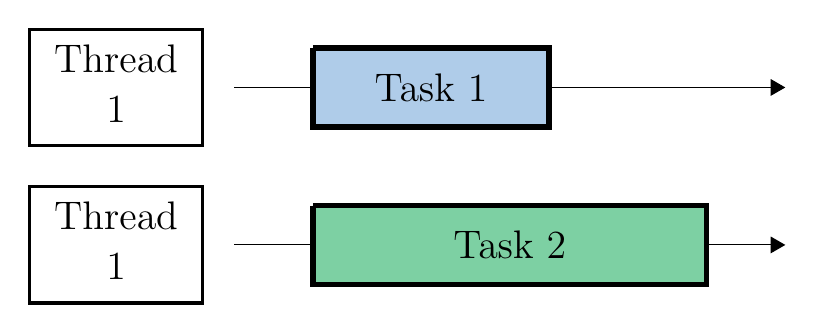
\begin{tikzpicture}
% 1. Place the CPU
\node[square] at (-3.5,1) {\begin{tabular}{c} Thread \\ 1 \end{tabular}};;

% 1. Place the CPU
\node[square] at (-3.5,-1) {\begin{tabular}{c} Thread \\ 1 \end{tabular}};;




\draw[-triangle 60]  (-2,1) -- node[pos=1, anchor=west] {\textbf{\begin{tabular}{c} \end{tabular}}}(5,1);
\draw[-triangle 60]  (-2,-1) -- node[pos=1, anchor=west] {\textbf{\begin{tabular}{c} \end{tabular}}}(5,-1);



%%% TASK 1
% Box with borders on top, left, bottom (no right)
\node[blue,anchor=west] (t2) at (-1,1) {Task 1};
\draw[black,line width=2] (t2.north west) -- (t2.north east) -- (t2.south east) -- (t2.south west) -- (t2.north west);



%%% TASK 2
% Box with borders on top, left, bottom (no right)
\node[green, anchor=west] (s2) at (-1,-1) {Task 2};
\draw[black,line width=2] (s2.north west) -- (s2.north east) -- (s2.south east) -- (s2.south west) -- (s2.north west);



\end{tikzpicture}

\end{document}
